% Options for packages loaded elsewhere
\PassOptionsToPackage{unicode}{hyperref}
\PassOptionsToPackage{hyphens}{url}
%
\documentclass[
]{book}
\usepackage{amsmath,amssymb}
\usepackage{lmodern}
\usepackage{iftex}
\ifPDFTeX
  \usepackage[T1]{fontenc}
  \usepackage[utf8]{inputenc}
  \usepackage{textcomp} % provide euro and other symbols
\else % if luatex or xetex
  \usepackage{unicode-math}
  \defaultfontfeatures{Scale=MatchLowercase}
  \defaultfontfeatures[\rmfamily]{Ligatures=TeX,Scale=1}
\fi
% Use upquote if available, for straight quotes in verbatim environments
\IfFileExists{upquote.sty}{\usepackage{upquote}}{}
\IfFileExists{microtype.sty}{% use microtype if available
  \usepackage[]{microtype}
  \UseMicrotypeSet[protrusion]{basicmath} % disable protrusion for tt fonts
}{}
\makeatletter
\@ifundefined{KOMAClassName}{% if non-KOMA class
  \IfFileExists{parskip.sty}{%
    \usepackage{parskip}
  }{% else
    \setlength{\parindent}{0pt}
    \setlength{\parskip}{6pt plus 2pt minus 1pt}}
}{% if KOMA class
  \KOMAoptions{parskip=half}}
\makeatother
\usepackage{xcolor}
\usepackage{longtable,booktabs,array}
\usepackage{calc} % for calculating minipage widths
% Correct order of tables after \paragraph or \subparagraph
\usepackage{etoolbox}
\makeatletter
\patchcmd\longtable{\par}{\if@noskipsec\mbox{}\fi\par}{}{}
\makeatother
% Allow footnotes in longtable head/foot
\IfFileExists{footnotehyper.sty}{\usepackage{footnotehyper}}{\usepackage{footnote}}
\makesavenoteenv{longtable}
\usepackage{graphicx}
\makeatletter
\def\maxwidth{\ifdim\Gin@nat@width>\linewidth\linewidth\else\Gin@nat@width\fi}
\def\maxheight{\ifdim\Gin@nat@height>\textheight\textheight\else\Gin@nat@height\fi}
\makeatother
% Scale images if necessary, so that they will not overflow the page
% margins by default, and it is still possible to overwrite the defaults
% using explicit options in \includegraphics[width, height, ...]{}
\setkeys{Gin}{width=\maxwidth,height=\maxheight,keepaspectratio}
% Set default figure placement to htbp
\makeatletter
\def\fps@figure{htbp}
\makeatother
\setlength{\emergencystretch}{3em} % prevent overfull lines
\providecommand{\tightlist}{%
  \setlength{\itemsep}{0pt}\setlength{\parskip}{0pt}}
\setcounter{secnumdepth}{5}
\ifLuaTeX
\usepackage[bidi=basic]{babel}
\else
\usepackage[bidi=default]{babel}
\fi
\babelprovide[main,import]{brazilian}
% get rid of language-specific shorthands (see #6817):
\let\LanguageShortHands\languageshorthands
\def\languageshorthands#1{}
\usepackage{booktabs}
\ifLuaTeX
  \usepackage{selnolig}  % disable illegal ligatures
\fi
\usepackage[]{natbib}
\bibliographystyle{plainnat}
\IfFileExists{bookmark.sty}{\usepackage{bookmark}}{\usepackage{hyperref}}
\IfFileExists{xurl.sty}{\usepackage{xurl}}{} % add URL line breaks if available
\urlstyle{same} % disable monospaced font for URLs
\hypersetup{
  pdftitle={Bookdown de Resumos de Livros ( Ciência da Computação )},
  pdfauthor={Daniel Claudino},
  pdflang={pt-BR},
  hidelinks,
  pdfcreator={LaTeX via pandoc}}

\title{Bookdown de Resumos de Livros ( Ciência da Computação )}
\author{Daniel Claudino}
\date{2022-11-18}

\begin{document}
\maketitle

{
\setcounter{tocdepth}{1}
\tableofcontents
}
\hypertarget{apresentauxe7uxe3o}{%
\chapter{Apresentação}\label{apresentauxe7uxe3o}}

\begin{figure}

{\centering 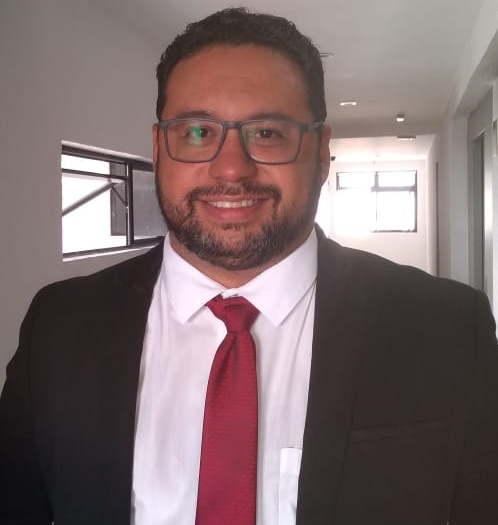
\includegraphics[width=0.5\linewidth]{imagens/FOTO-PERFIL-DANIEL-CLAUDINO-2020} 

}

\caption{Autor}\label{fig:unnamed-chunk-1}
\end{figure}

durante minha formação acadêmica, bacharelado, mestrado e doutorado.

\hypertarget{como-este-bookdown-estuxe1-organizado}{%
\section{Como Este Bookdown Está Organizado ?}\label{como-este-bookdown-estuxe1-organizado}}

Cada capítulo deste bookdown corresponderá a um livro ( nível \# ).

Dentro de cada capítulo deste bookdown ( nível \# ), colocarei os resumos dos capítulos do livro correspondente no nível 2 ( \# \# ).

As seções de cada capítulo do livro resumido estarão nos níveis 3 e 4 ( \# \# \# e \# \# \# \# ) de cada capítulo deste bookdown.

\hypertarget{controle-de-versuxe3o}{%
\section{Controle de Versão}\label{controle-de-versuxe3o}}

\begin{longtable}[]{@{}
  >{\raggedright\arraybackslash}p{(\columnwidth - 6\tabcolsep) * \real{0.2500}}
  >{\raggedright\arraybackslash}p{(\columnwidth - 6\tabcolsep) * \real{0.2500}}
  >{\raggedright\arraybackslash}p{(\columnwidth - 6\tabcolsep) * \real{0.2500}}
  >{\raggedright\arraybackslash}p{(\columnwidth - 6\tabcolsep) * \real{0.2500}}@{}}
\toprule()
\begin{minipage}[b]{\linewidth}\raggedright
Versão
\end{minipage} & \begin{minipage}[b]{\linewidth}\raggedright
Data / Hora
\end{minipage} & \begin{minipage}[b]{\linewidth}\raggedright
Colaborador
\end{minipage} & \begin{minipage}[b]{\linewidth}\raggedright
Descrição da Contribuição
\end{minipage} \\
\midrule()
\endhead
0.1 & dd/mm/aaaa xxh00 & \href{https://wa.me/5583988853815}{Daniel Claudino} & Versão inicial do documento \\
\bottomrule()
\end{longtable}

\hypertarget{livro-engenharia-de-software-sommervile-2007}{%
\chapter{Livro: Engenharia de Software (Sommervile, 2007)}\label{livro-engenharia-de-software-sommervile-2007}}

\begin{figure}

{\centering 
\includegraphics[width=0.5\linewidth]{imagens/livro_capa_sommerville2007} 

}

\caption{Livro: Engenharia de Software (Sommervile, 2007)}\label{fig:unnamed-chunk-2}
\end{figure}

\hypertarget{parte-2---requisitos-capuxedtulo-6---requisitos-de-software}{%
\section{Parte 2 - Requisitos ( Capítulo 6 - Requisitos de Software )}\label{parte-2---requisitos-capuxedtulo-6---requisitos-de-software}}

\begin{itemize}
\tightlist
\item
  O QUE É a \textbf{engenharia de requisitos} ?

  \begin{itemize}
  \tightlist
  \item
    É um processo de comunicação

    \begin{itemize}
    \tightlist
    \item
      Entre clientes, usuários e desenvolvedores
    \end{itemize}
  \item
    NÃO É simplesmente um processo técnico
  \end{itemize}
\item
  Com o que a \textbf{engenharia de requisitos} ESTÁ RELACIONADA ?

  \begin{itemize}
  \tightlist
  \item
    ESTÁ RELACIONADA com O QUE o sistema irá fazer;
  \item
    ESTÁ RELACIONADA com a definição das PROPRIEDADES EMERGENTES do sistema

    \begin{itemize}
    \tightlist
    \item
      Propriedades emergentes ESSENCIAIS
    \item
      Propriedades emergentes DESEJÁVEIS
    \end{itemize}
  \item
    ESTA RELACIONADA com as RESTRIÇÕES do sistema

    \begin{itemize}
    \tightlist
    \item
      Restrições quanto A OPERAÇÃO
    \item
      Restrição quanto AO PROCESSO DE DESENVOLVIMENTO DE SOFTWARE
    \end{itemize}
  \end{itemize}
\item
  A \textbf{PARTE 2} do livro trata:

  \begin{itemize}
  \tightlist
  \item
    Das \textbf{BASES} DA ENGENHARIA DE SOFTWARE ( Capítulos 6 e 7 )

    \begin{itemize}
    \tightlist
    \item
      \textbf{Requisitos de Software}

      \begin{enumerate}
      \def\labelenumi{\arabic{enumi}.}
      \tightlist
      \item
        o que são requisitos ?
      \item
        Quais os tipos de requisitos ?
      \item
        Como os requistios devem ser organizados ?
      \end{enumerate}
    \item
      \textbf{Atividades do Processo de Software}

      \begin{enumerate}
      \def\labelenumi{\arabic{enumi}.}
      \tightlist
      \item
        Estudos de viabilidade;
      \item
        Técnicas de \textbf{elicitação} de requisitos;
      \item
        Técnicas de \textbf{análise} de requisitos;
      \item
        \textbf{Validação} de requisitos;
      \end{enumerate}
    \end{itemize}
  \item
    Da DESCRIÇÃO DOS \textbf{MODELOS} E \textbf{TÉCNICAS} ( Capítulos 8 e 9 )

    \begin{itemize}
    \tightlist
    \item
      Tipos de modelos de sistemas

      \begin{enumerate}
      \def\labelenumi{\arabic{enumi}.}
      \tightlist
      \item
        Modelagem orientada a objeto
      \end{enumerate}
    \item
      Especificação de sistemas críticos

      \begin{enumerate}
      \def\labelenumi{\arabic{enumi}.}
      \tightlist
      \item
        Propriedades emergentes \textbf{de confiança}
      \item
        Abordagem \textbf{dirigida a riscos}
      \item
        Tópicos específicos de \textbf{especificação}:

        \begin{enumerate}
        \def\labelenumii{\alph{enumii}.}
        \tightlist
        \item
          De \textbf{segurança}
        \item
          De \textbf{confiança}
        \item
          De \textbf{proteção}
        \end{enumerate}
      \item
        Técnicas e métodos formais de especificação de requisitos
      \end{enumerate}
    \end{itemize}
  \end{itemize}
\end{itemize}

\hypertarget{quais-os-objetivos-deste-capuxedtulo}{%
\subsection*{Quais os objetivos deste capítulo ?}\label{quais-os-objetivos-deste-capuxedtulo}}
\addcontentsline{toc}{subsection}{Quais os objetivos deste capítulo ?}

\begin{itemize}
\tightlist
\item
  Apresentar os requisitos de sistemas de software;
\item
  Explicar diferentes modos de expressar os requisitos de software.
\end{itemize}

\hypertarget{quais-as-competuxeancias-esperadas-ao-final-do-capuxedtulo}{%
\subsection*{Quais as competências esperadas ao final do capítulo ?}\label{quais-as-competuxeancias-esperadas-ao-final-do-capuxedtulo}}
\addcontentsline{toc}{subsection}{Quais as competências esperadas ao final do capítulo ?}

\begin{enumerate}
\def\labelenumi{\arabic{enumi}.}
\tightlist
\item
  CONHECIMENTO a respeito dos conceitos de:
\end{enumerate}

\begin{itemize}
\tightlist
\item
  Requisitos de usuário;
\item
  Requisitos de sistema;
\end{itemize}

\begin{enumerate}
\def\labelenumi{\arabic{enumi}.}
\setcounter{enumi}{1}
\tightlist
\item
  CONHECIMENTO do porquê da necessidade de expressar (escrever) de forma diferente os requisitos funcionais e os requisitos não funcionais
\item
  HABILIDADE de organizar os requisitos em um *DOCUMENTO DE REQUISITOS DE SOFTWARE**
\end{enumerate}

\hypertarget{requisitos-de-software}{%
\subsection{Requisitos de Software}\label{requisitos-de-software}}

\begin{itemize}
\tightlist
\item
  \textbf{Requisitos} de software são:

  \begin{enumerate}
  \def\labelenumi{\arabic{enumi}.}
  \tightlist
  \item
    \textbf{DESCRIÇÃO DOS SERVIÇOS} fornecidos pelo sistema;
  \item
    As \textbf{RESTRIÇÕES} operacionais do sistema
  \end{enumerate}
\item
  \textbf{Engenharia de requisitos} (RE - Requirements Engineering) é o \textbf{processo} de:

  \begin{itemize}
  \tightlist
  \item
    Descobrir serviços e restrições de software;
  \item
    Analisar serviços e restrições de software;
  \item
    Documentar serviços e restrições de software;
  \item
    Verificar serviços e restrições de software;
  \end{itemize}
\end{itemize}

\hypertarget{requisitos-funcionais-e-nuxe3o-funcionais}{%
\subsection{Requisitos funcionais e Não Funcionais}\label{requisitos-funcionais-e-nuxe3o-funcionais}}

Lorem ipsum. Lorem ipsum. Lorem ipsum. Lorem ipsum. Lorem ipsum. Lorem ipsum. Lorem ipsum. Lorem ipsum. Lorem ipsum. Lorem ipsum. Lorem ipsum. Lorem ipsum. Lorem ipsum. Lorem ipsum. Lorem ipsum. Lorem ipsum. Lorem ipsum. Lorem ipsum. Lorem ipsum.

\hypertarget{requisitos-de-usuuxe1rio}{%
\subsection{Requisitos de usuário}\label{requisitos-de-usuuxe1rio}}

Lorem ipsum. Lorem ipsum. Lorem ipsum. Lorem ipsum. Lorem ipsum. Lorem ipsum. Lorem ipsum. Lorem ipsum. Lorem ipsum. Lorem ipsum. Lorem ipsum. Lorem ipsum. Lorem ipsum. Lorem ipsum. Lorem ipsum. Lorem ipsum. Lorem ipsum. Lorem ipsum. Lorem ipsum.

\hypertarget{requisitos-de-sistema}{%
\subsection{Requisitos de sistema}\label{requisitos-de-sistema}}

Lorem ipsum. Lorem ipsum. Lorem ipsum. Lorem ipsum. Lorem ipsum. Lorem ipsum. Lorem ipsum. Lorem ipsum. Lorem ipsum. Lorem ipsum. Lorem ipsum. Lorem ipsum. Lorem ipsum. Lorem ipsum. Lorem ipsum. Lorem ipsum. Lorem ipsum. Lorem ipsum. Lorem ipsum.

\hypertarget{especificauxe7uxe3o-de-interface}{%
\subsection{Especificação de interface}\label{especificauxe7uxe3o-de-interface}}

Lorem ipsum. Lorem ipsum. Lorem ipsum. Lorem ipsum. Lorem ipsum. Lorem ipsum. Lorem ipsum. Lorem ipsum. Lorem ipsum. Lorem ipsum. Lorem ipsum. Lorem ipsum. Lorem ipsum. Lorem ipsum. Lorem ipsum. Lorem ipsum. Lorem ipsum. Lorem ipsum. Lorem ipsum.

\hypertarget{documento-de-requisito-de-software-drs}{%
\subsection{Documento de requisito de software (DRS)}\label{documento-de-requisito-de-software-drs}}

Lorem ipsum. Lorem ipsum. Lorem ipsum. Lorem ipsum. Lorem ipsum. Lorem ipsum. Lorem ipsum. Lorem ipsum. Lorem ipsum. Lorem ipsum. Lorem ipsum. Lorem ipsum. Lorem ipsum. Lorem ipsum. Lorem ipsum. Lorem ipsum. Lorem ipsum. Lorem ipsum. Lorem ipsum.

\hypertarget{pontos-chave-leituras-sugeridas-e-exercuxedcios}{%
\subsection*{Pontos chave, leituras sugeridas e exercícios}\label{pontos-chave-leituras-sugeridas-e-exercuxedcios}}
\addcontentsline{toc}{subsection}{Pontos chave, leituras sugeridas e exercícios}

Lorem ipsum. Lorem ipsum. Lorem ipsum. Lorem ipsum. Lorem ipsum. Lorem ipsum. Lorem ipsum. Lorem ipsum. Lorem ipsum. Lorem ipsum. Lorem ipsum. Lorem ipsum. Lorem ipsum. Lorem ipsum. Lorem ipsum. Lorem ipsum. Lorem ipsum. Lorem ipsum. Lorem ipsum.

\hypertarget{nome-do-produto-da-disciplina-nome-da-disciplina}{%
\chapter{NOME-DO-PRODUTO da Disciplina NOME-DA-DISCIPLINA}\label{nome-do-produto-da-disciplina-nome-da-disciplina}}

Neste capítulo estarão contidos os NOME-DO-PRODUTO da disciplina NOME-DA-DISCIPLINA.

\begin{longtable}[]{@{}ll@{}}
\toprule()
Data & Tópicos Abordados \\
\midrule()
\endhead
dd/mm/aaaa & - Tópico 1- Tópico 2- Tópico 3 \\
\bottomrule()
\end{longtable}

\hypertarget{seuxe7uxe3o-01}{%
\section{Seção 01}\label{seuxe7uxe3o-01}}

\hypertarget{subseuxe7uxe3o-numerada-1}{%
\subsection{Subseção Numerada 1}\label{subseuxe7uxe3o-numerada-1}}

Lorem ipsum. Lorem ipsum. Lorem ipsum. Lorem ipsum. Lorem ipsum. Lorem ipsum. Lorem ipsum. Lorem ipsum. Lorem ipsum. Lorem ipsum. Lorem ipsum. Lorem ipsum. Lorem ipsum. Lorem ipsum. Lorem ipsum. Lorem ipsum. Lorem ipsum. Lorem ipsum. Lorem ipsum.

\hypertarget{subseuxe7uxe3o-numerada-2}{%
\subsection{Subseção Numerada 2}\label{subseuxe7uxe3o-numerada-2}}

Lorem ipsum. Lorem ipsum. Lorem ipsum. Lorem ipsum. Lorem ipsum. Lorem ipsum. Lorem ipsum. Lorem ipsum. Lorem ipsum. Lorem ipsum. Lorem ipsum. Lorem ipsum. Lorem ipsum. Lorem ipsum. Lorem ipsum. Lorem ipsum. Lorem ipsum. Lorem ipsum. Lorem ipsum.

\hypertarget{seuxe7uxe3o-nuxe3o-numerada-3}{%
\subsection*{Seção não Numerada 3}\label{seuxe7uxe3o-nuxe3o-numerada-3}}
\addcontentsline{toc}{subsection}{Seção não Numerada 3}

Lorem ipsum. Lorem ipsum. Lorem ipsum. Lorem ipsum. Lorem ipsum. Lorem ipsum. Lorem ipsum. Lorem ipsum. Lorem ipsum. Lorem ipsum. Lorem ipsum. Lorem ipsum. Lorem ipsum. Lorem ipsum. Lorem ipsum. Lorem ipsum. Lorem ipsum. Lorem ipsum. Lorem ipsum.

\hypertarget{seuxe7uxe3o-02}{%
\section{Seção 02}\label{seuxe7uxe3o-02}}

\hypertarget{subseuxe7uxe3o-numerada-1-1}{%
\subsection{Subseção Numerada 1}\label{subseuxe7uxe3o-numerada-1-1}}

Lorem ipsum. Lorem ipsum. Lorem ipsum. Lorem ipsum. Lorem ipsum. Lorem ipsum. Lorem ipsum. Lorem ipsum. Lorem ipsum. Lorem ipsum. Lorem ipsum. Lorem ipsum. Lorem ipsum. Lorem ipsum. Lorem ipsum. Lorem ipsum. Lorem ipsum. Lorem ipsum. Lorem ipsum.

\hypertarget{subseuxe7uxe3o-numerada-2-1}{%
\subsection{Subseção Numerada 2}\label{subseuxe7uxe3o-numerada-2-1}}

Lorem ipsum. Lorem ipsum. Lorem ipsum. Lorem ipsum. Lorem ipsum. Lorem ipsum. Lorem ipsum. Lorem ipsum. Lorem ipsum. Lorem ipsum. Lorem ipsum. Lorem ipsum. Lorem ipsum. Lorem ipsum. Lorem ipsum. Lorem ipsum. Lorem ipsum. Lorem ipsum. Lorem ipsum.

\hypertarget{seuxe7uxe3o-nuxe3o-numerada-3-1}{%
\subsection*{Seção não Numerada 3}\label{seuxe7uxe3o-nuxe3o-numerada-3-1}}
\addcontentsline{toc}{subsection}{Seção não Numerada 3}

Lorem ipsum. Lorem ipsum. Lorem ipsum. Lorem ipsum. Lorem ipsum. Lorem ipsum. Lorem ipsum. Lorem ipsum. Lorem ipsum. Lorem ipsum. Lorem ipsum. Lorem ipsum. Lorem ipsum. Lorem ipsum. Lorem ipsum. Lorem ipsum. Lorem ipsum. Lorem ipsum. Lorem ipsum.

\begin{itemize}
\tightlist
\item
\end{itemize}

  \bibliography{referencias.bib,packages.bib}

\end{document}
